In this chapter we will describe: 
\begin{itemize}
	\item How the graph representing the environment is generated.
	\item The heuristic we use in A*.
\end{itemize}
A class diagram about all of the classes that are relevant to the path planning can be found at the bottom of this chapter.
\subsubsection{Generation of the graph}
Our game consists of a tile system. The Game world is divided into a 40x40 grid of tiles and each buildable tile has it's own vertex. The vertex of a tile is connected to the vertexes of neighbouring tiles by Edges, creating a graph.
\begin{figure}[H]
	\centering
	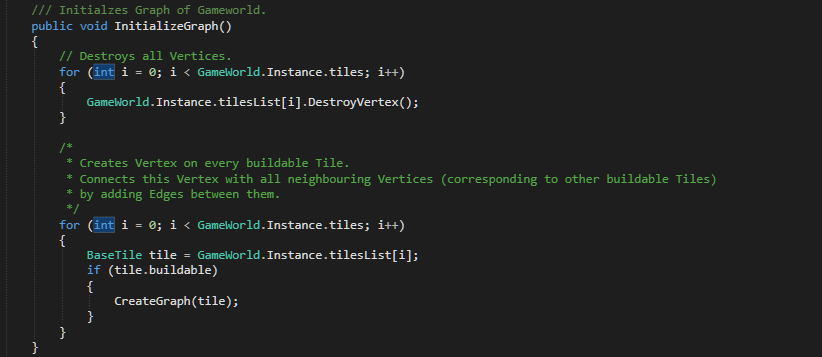
\includegraphics[width=\linewidth]{Images/graphgeneration1}
	\caption{How the graph of the Gameworld is generated.}
	\label{fig:graphgeneration1}
\end{figure} 
\begin{figure}[H]
	\centering
	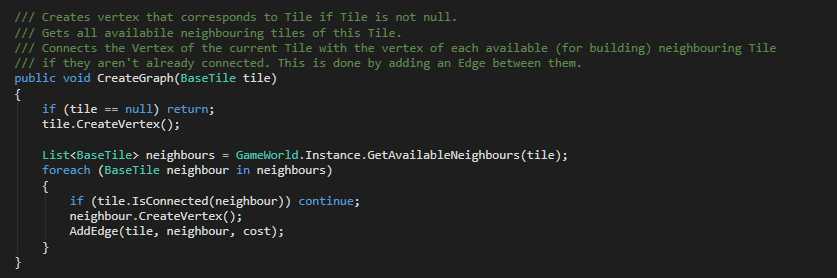
\includegraphics[width=1\linewidth]{Images/graphgeneration2}
	\caption{CreateGraph method.}
	\label{fig:graphgeneration2}
\end{figure} 
\subsubsection{Heuristic}
We use the Manhattan heuristic for calculating the distance between two tiles.
\begin{figure}[H]
	\centering
	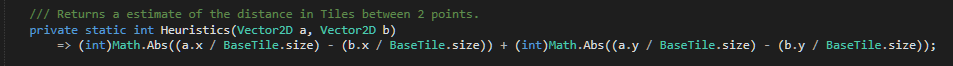
\includegraphics[width=1\linewidth]{Images/heuristics}
	\caption{Function for calculating Manhattan distance between two points.}
	\label{fig:heuristics}
\end{figure} 
\subsubsection{Class Diagram}
\begin{figure}[H]
	\centering
	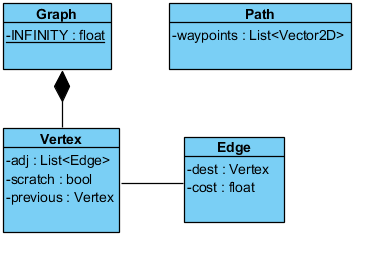
\includegraphics[width=\linewidth]{Images/pathplanningclassdiagram}
	\caption{Class diagram of classes that are relevant to path planning.}
	\label{fig:pathplanningclassdiagram}
\end{figure}